\testCom
{%Номер задачи
	3.141
}
{%Условие
	условие
}
{%Дано
	дано
}
{%Найти
	найти
}
{%Решение
	Запишем закон Ома и правило Киргофа:\\
	$\begin{cases}
		L_1 \der{I_1}{t}{} + I_1 R_1 = L_2 \der{I_2}{t}{} + I_2 R_2 = L \der{I}{t}{} + IR & I_1 = \der{q_1}{t}{} I_2 = \der{q_2}{t}{}\\
		I = I_1 + I_2 & то \, \der{q}{t}{} = I
	  \end{cases}$\\
	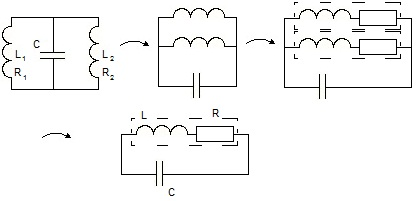
\includegraphics[height=40mm]{3_141.jpg}\\
	$L \der{I}{t}{} = L_1 \der{I_1}{t}{} = L_2 \der{I_2}{t}{}, \quad \der{I_1}{t}{} + \der{I_2}{t}{} = \der{I}{t}{} \Rightarrow \frac{1}{L} = \frac{1}{L_1} + \frac{1}{L_2} $\\
	$RI = I_1 R_1 = I_2 R_2 , I_1 + I_2 = I \Rightarrow \frac{1}{R} = \frac{1}{R_1} + \frac{1}{R_2}$\\
}

